\documentclass{report}
\usepackage[T1]{fontenc} % Fontes T1
\usepackage[utf8]{inputenc} % Input UTF8
\usepackage[backend=biber, style=ieee]{biblatex} % para usar bibliografia
\usepackage{csquotes}
\usepackage[portuguese]{babel} %Usar língua portuguesa
\usepackage{blindtext} % Gerar texto automaticamente
\usepackage[printonlyused]{acronym}
\usepackage{hyperref} % para autoref
\usepackage{graphicx}
\usepackage{placeins}

\bibliography{bibliografia}


\begin{document}
%%
% Definições
%
\def\titulo{SERVIDOR DE CAIXAS SEGURAS}
\def\subtitulo{CLIENTE, TESTES & DOCUMENTOS}
\def\data{21 de ABRIL de 2017}
\def\autores{Rafael Santos, Paulo Vasconcelos}
\def\autorescontactos{(84951) r.c.santos@ua.pt, (84987) paulobvasconcelos@ua.pt}
\def\versao{LABORATÓRIOS DE INFORMÁTICA}
\def\departamento{DETI}
\def\empresa{UNIVERSIDADE DE AVEIRO}
\def\logotipo{ua.pdf}
%
%%%%%% CAPA %%%%%%
%
\begin{titlepage}

\begin{center}
%
\vspace*{50mm}
%
{\Huge \titulo}\\ 
%
\vspace{10mm}
%
{\Large \empresa}\\
%
\vspace{10mm}
%
{\LARGE \autores}\\ 
%
\vspace{30mm}
%
\begin{figure}[h]
\center
\includegraphics{\logotipo}
\end{figure}
%
\vspace{30mm}
\end{center}
%
\begin{flushright}
\versao
\end{flushright}
\end{titlepage}

%%  Página de Título %%
\title{%
{\Huge\textbf{\titulo}}\\
{\Large \departamento\\ \empresa}
}
%
\author{%
    \autores \\
    \autorescontactos
}
%
\date{\data}
%
\maketitle

\pagenumbering{roman}

%%%%%% RESUMO %%%%%%
\begin{abstract}
Este relatório tem como principal objetivo enquadrar o trabalho de implementação da ligação entre o cliente e o servidor (\textit{xcoa}).

\end{abstract}

%%%%%% Agradecimentos %%%%%%
% Segundo glisc deveria aparecer após conclusão...
%\renewcommand{\abstractname}{Agradecimentos}
%\begin{abstract}
%Eventuais agradecimentos.
%Comentar bloco caso não existam agradecimentos a fazer.
%\end{abstract}


\tableofcontents
% \listoftables     % descomentar se necessário
\listoffigures    % descomentar se necessário


%%%%%%%%%%%%%%%%%%%%%%%%%%%%%%%
\clearpage
\pagenumbering{arabic}

%%%%%%%%%%%%%%%%%%%%%%%%%%%%%%%%
\chapter{Introdução}
\label{chap.introducao}

Das últimas décadas a esta parte, "globalização" tem sido a palavra-chave.
Este processo de aproximação de toda a população foi impulsionado pelo desenvolvimento de tecnologias que permitem uma comunicação rápida e eficaz a longas distancias, como é o caso da Inernet. \br
Com o passar do tempo, foi possivel transmitir mais informação de maneira mais rápida, o que eventualmente levou ao surgimento de questões relativas à segurança e privacidade dos utilizadores destas tecnologias.

Foi com o intuito de conhecer as dificuldades que são apresentadas no estabelecimento de ligações a longas distancias que este trabalho foi realizado. Neste trabalho, foi realizada uma ligação ao server do (\textit{xcoa}) onde foi implementado um programa de um modelo de caixas seguras, o qual será explicado mais adiante, que irá interagir com o programa desenvolvido.

Este documento está dividido em quatro capítulos.
Depois desta introdução,
no \autoref{chap.pesquisa} são apresentadas algumas noções básicas de criptografia.,
no \autoref{chap.metodologia} é apresentada a metodologia seguida e as funções desenvolvidas juntamente com a utilização de cada uma,
no \autoref{chap.conclusao} são apresentadas
as conclusões do trabalho aquando da aplicação do cliente desenvolvido.
Finalmente, no \autoref{chap.contribuicao} são explicitadas as contribuições de cada um dos autores para o trabalho e as percentagens atribuidas a cada um conforme os resultados apresentados.


\chapter{Pesquisa}
\label{chap.pesquisa}

Criptografia.
Por definição é \textit{o estudo dos princípios e técnicas pelas quais a informação pode ser transformada da sua forma original para outra, ilegível, de forma a que possa ser conhecida apenas pelo seu destinatário, o que torna difícil a sua leitura por alguém não autorizado.}.
Na prática, é o que permite haver confidencialidade na internet (e não só).

No mundo de hoje, são facilmente identificáveis os dois sistemas básicos de criptografia existentes: sistemas \textbf{simétricos} e \textbf{assimétricos}.

No sistema simétrico, a chave que realiza a encriptação é a mesma que realiza a desencriptação pelo que a sua segurança é fulcral.

Num sistema assimétrico, cada utilizador possui duas chaves. Uma pública e outra privada.
A chave pública é utilizada para encriptar todas as mensagens que o utilizador irá receber e a sua chave privada desencriptará essas mesmas mensagens.
A chave pública é dada a conhecer a todos os utilizadores para que seja possível o envio de mensagens à entidade portadora dessa mesma chave.
A chave privada é apenas conhecida pelo próprio utilizador pois qualquer utilizador com acesso à mesma será capaz de desencriptar as mensagens obtendo assim o acesso a informação potencialmente privada.

\FloatBarrier
\chapter{Metodologia}
\label{chap.metodologia}
\section{Comandos Pre Main}

Antes de ser executada a função \textit{main}, são executados vários comandos que permitem o bom funcionamento do código.\br
O primeiro comando apresentado, \textit{gen\_key}, verifica se existe um par de chaves \textit{RSA} já gerado, e, caso não exista, gera um novo par de chaves que irá ser usado nas funções \textit{CREATE} (nas criação de caixas privadas) e \textit{GET}.


\begin{figure}[h]
\center
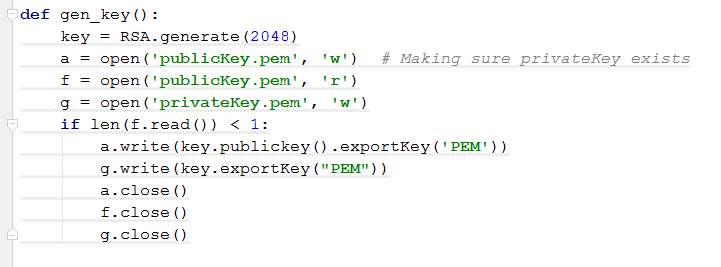
\includegraphics[width=400pt]{gen_key}
\caption{Função \textit{gen\_key}}
\label{fig:gen_key}
\end{figure}


Seguidamente, tem-se a criação dos \textit{sockets} e a ligação ao \textit{server}. Antes de se efetuar uma ligação definitiva ao mesmo, faz-se um teste de ligação ao \textit{server} e, caso não reponda (por o utilizador não estar ligado à Internet ou o \textit{server} estar em baixo), mostra uma mensagem de erro e seguidamente fecha o programa.\br
Caso a ligação seja corretamente realizada, é apresentado um menu com as opções que o utilizador pode escolher atraves da introdução de texto pelo teclado.

\begin{figure}[h]
\center
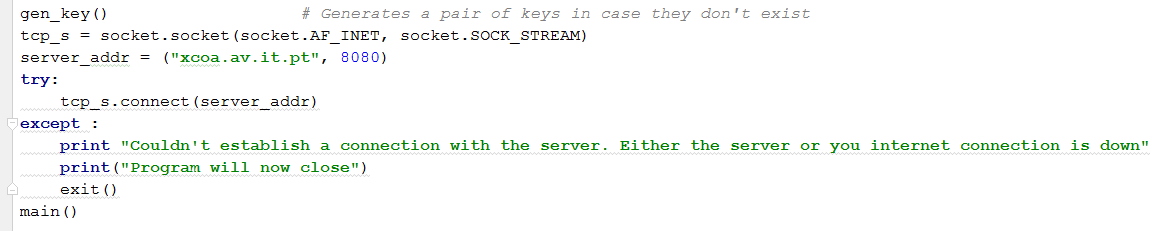
\includegraphics[width=400pt]{general}
\caption{Exceções}
\label{fig:general}
\end{figure}


\FloatBarrier
\section{Funções}
Irá agora ser apresentada uma descrição de cada função do programa.

\begin{figure}[h]
\center
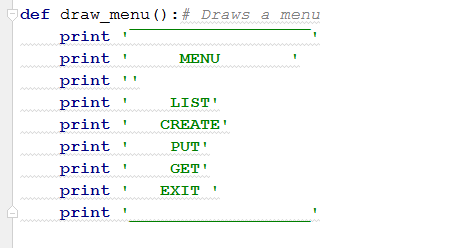
\includegraphics[width=400pt]{draw_menu}
\caption{Função \textit{draw\_menu}}
\label{fig:draw_menu}
\end{figure}

\newpage
\FloatBarrier
\subsection{MAIN}

Na função \textit{Main}, é definida a estrutura geral do programa.
Começa por definir se o programa vai funcionar apenas com base num menu, ou se cada função deve ser executada diretamente a partir do terminal. Como tal, a função \textit{main} começa por ver se existem argumentos adicionais fornecidos ao programa. Caso existam, executa a função correspondente aos argumentos fornecidos. Caso sejam fornecidos argumentos inválidos, o programa apresenta uma mensagem de erro e encerra. Caso contrário, o programa executa normalmente.

Caso não sejam fornecidos argumentos adicionais ao programa, o programa mostra um menu e várias opções para o utilizador escolher. Caso o utilizador insira um comado inválido no programa, este mostra uma mensagem de erro e volta a mostrar o menu. O programa neste caso só termina se o utilizador inserir o comando \textit{EXIT} ou se forçar o encerramento do programa.

\begin{figure}[h]
\center
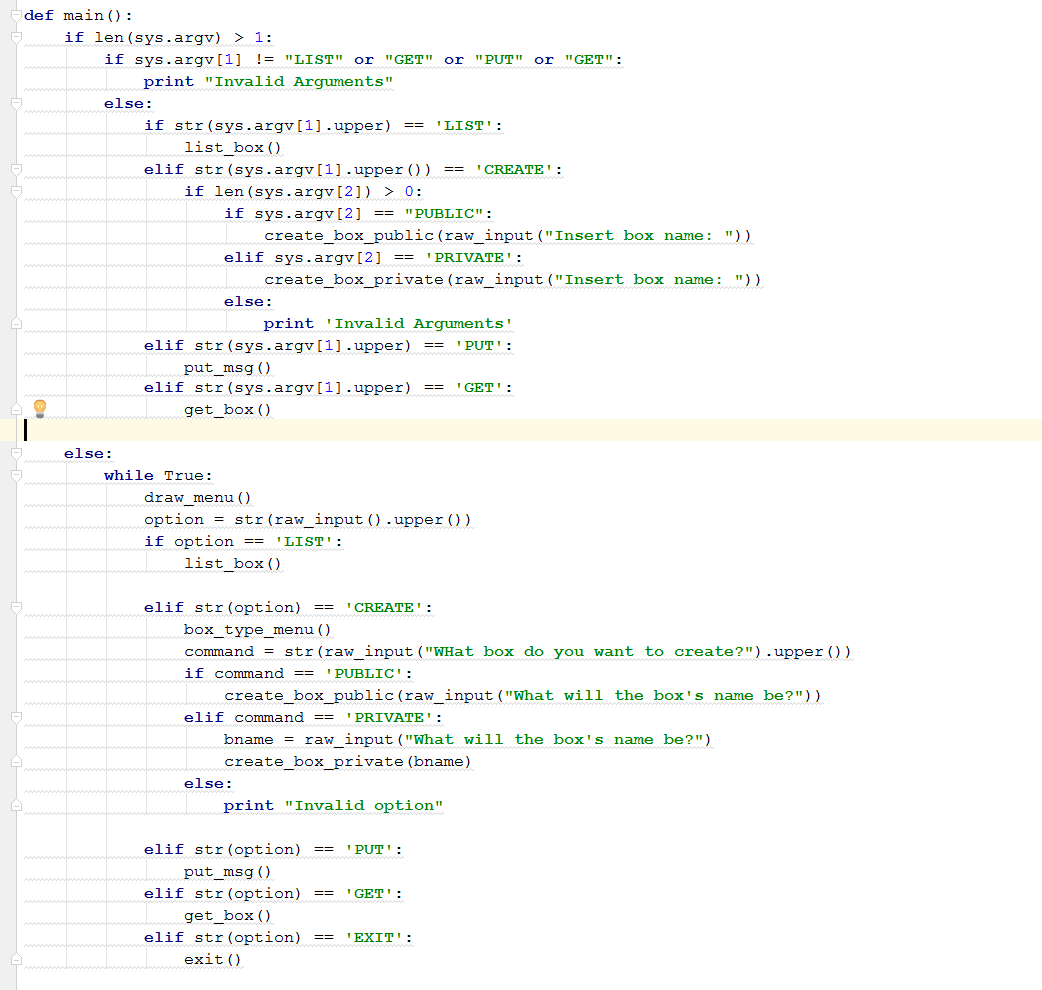
\includegraphics[width=400pt]{main}
\caption{Função \textit{main}}
\label{fig:main}
\end{figure}

\newpage
\FloatBarrier
\subsection{LIST}

No módulo \textit{lis1\_box}: 
\begin{figure}[h]
\center
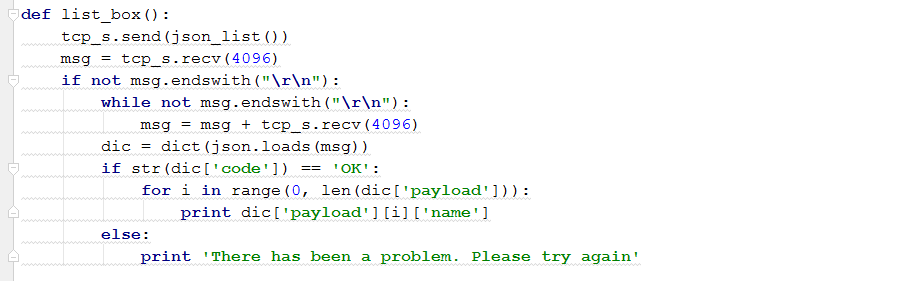
\includegraphics[width=400pt]{list_box}
\caption{Função \textit{list\_box}}
\label{fig:list_box}
\end{figure}
é enviada para o \textit{server} uma \textit{string} de \textit{JSON} terminada em \textbackslash r \textbackslash n (isto é necessario para o \textit{server} saber quando é que acabou o envio de informação) a qual é gerada através do módulo \textit{json\_list}:

\FloatBarrier
\begin{figure}[h]
\center
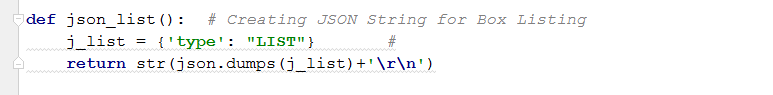
\includegraphics[width=400pt]{json_list}
\caption{Função \textit{json\_list}}
\label{fig:json_list}
\end{figure}

Apos ser gerada a \textit{string} de \textit{JSON} , é enviada ao server pelo \textit{socket}. Entretanto, o \textit{socket} aguarda por uma resposta por parte do \textit{server} acabada em \textbackslash r \textbackslash n apresentando depois uma listagem do nome de todas caixas que existem no \textit{server} ao utilizador.

\newpage
\FloatBarrier
\subsection{CREATE}
Nesta função, vão ser criadas as caixas que irão depois ficar armazenadas no \textit{server}. É de destacar que existem 2 tipos de caixas: caixas públicas e caixas privadas, sendo fornecido um menu que permite ao utilizador escolher o tipo de caixa que pretende criar.

\begin{figure}[h]
\center
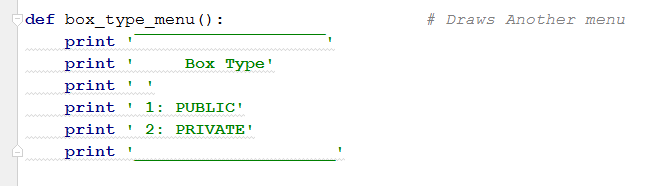
\includegraphics[width=400pt]{box_type_menu}
\caption{Função \textit{box\_type\_menu}}
\label{fig:box_type_menu}
\end{figure}
\subsubsection{Caixas Públicas}

As caixas públicas são criadas através do método \textit{create\_box\_public} que pede um argumento \textit{box\_name} que é pedido ao utilizador na execução da função \textit{main}.

\begin{figure}[h]
\center
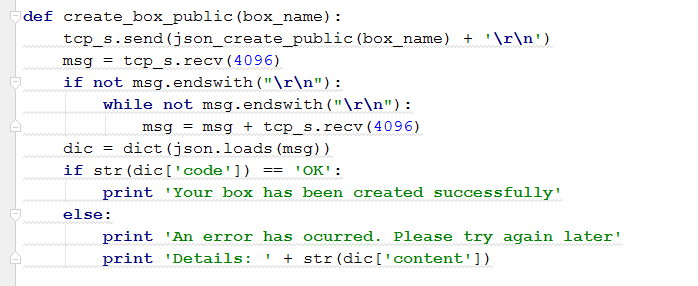
\includegraphics[width=400pt]{create_box_public}
\caption{Função \textit{create\_box\_public}}
\label{fig:create_box_public}
\end{figure}

É também definida uma string de \textit{JSON} através do método \textit{json\_create\_public(box\_name)}.
Após isto, é enviada a string de \textit{JSON}, com os campos relativos ao tipo de função que vai ser executada \textit{(type)}, o nome da caixa \textit{(name)} e o tempo em segundos \textit{(timestamp)} e e o socket espera por uma resposta do server que acabe em \textbackslash r \textbackslash n, que sinaliza o fim de envio de dados por parte do \textit{server}. Recebidos os dados, o programa apresenta uma mensagem de sucesso caso a caixa tenha sida criada. Caso contrário, apresenta uma mensagem de erro com detalhes sobre a razão da criação da caixa ter falhado.
\subsubsection{Caixas Privadas}
Nesta função vão ser criadas as caixas privadas, que podem apenas ser acedidas por quem criou a caixa. Para que tal seja possivel, é necessário o uso de criptografia (neste caso, segundo um sistema assimétrico). 

\begin{figure}[h]
\center
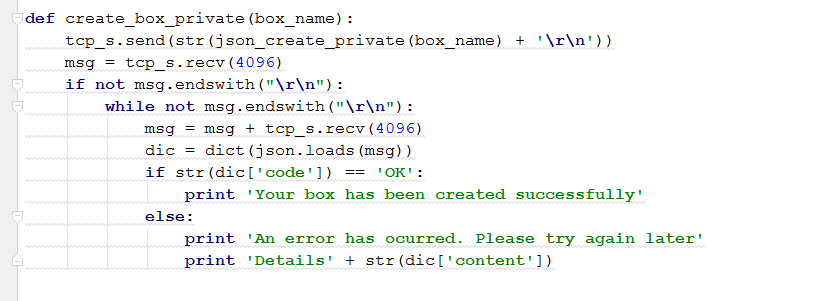
\includegraphics[width=400pt]{create_box_private}
\caption{Função \textit{create\_box\_private}}
\label{fig:create_box_private}
\end{figure}

A \textit{string} de \textit{JSON} para ser enviada ao server é produzida pelo módulo \textit{\_create\_private} que leva como argumento a variável box\_name e cria um documento em \textit{JSON} com campos relativos ao tipo de função que vai ser executada \textit{(type)}, o nome da caixa \textit{(name)}, a hora em segundos em que o pedido foi enviado  \textit{(timestamp)}, a chave pública relativa ao utilizador (\textit{pubk}) e a assinatura do utilizador (\textit{sig}) que é definida pelo pelo método de assinaturas \textit{PKCS1\_PSS}, com assinatura definida pela concatenação da \textit{timestamp} e do nome da caixa com o uso da chave privada do utilizador.

\begin{figure}[h]
\center
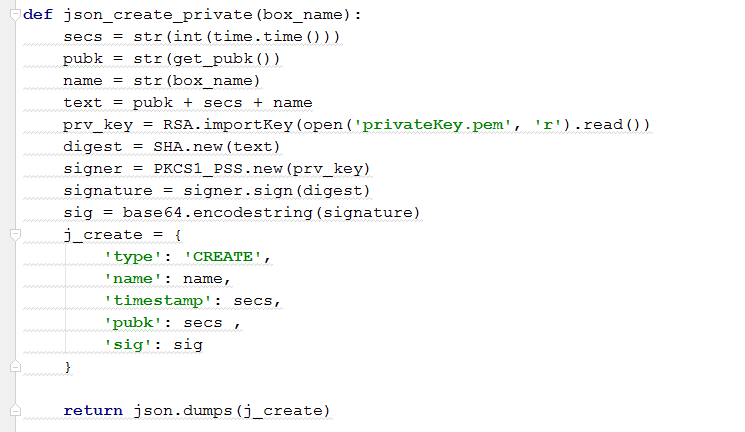
\includegraphics[width=400pt]{json_create_private}
\caption{Função \textit{json\_create_private}}
\label{fig:json_create_private}
\end{figure}

Após isto, a socket vai enviar a \textit{string} de \textit{JSON} acabada em \textbackslash r \textbackslashn e vai aguardar por uma resposta do server também acabada em \textbackslash r \textbackslash n, e após receber a resposta, apresenta ao utilizador uma mensagem de sucesso caso a caixa tenha sido criada, e caso contrário, mostra uma mensagem de erro com detalhes sobre o porquê de não ter sido possivel criar a caixa.

\begin{figure}[h]
\center
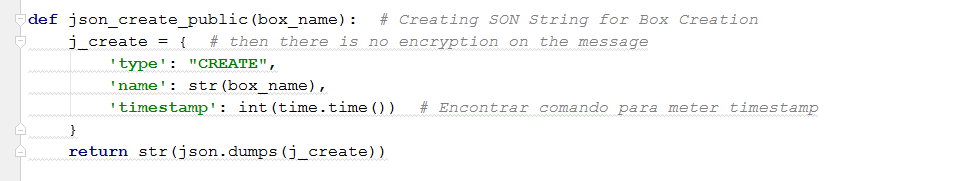
\includegraphics[width=400pt]{json_create_public}
\caption{Função \textit{json\_create_public}}
\label{fig:json_create_public}
\end{figure}


\newpage
\FloatBarrier
\subsection{PUT}
A função \textit{PUT} envia uma mensagem para um caixa, quer esta seja pública ou privada, tendo a particularidade de que apenas quem criou a caixa pode ver o seu conteúdo. Para isto, tem-se o módulo \textit{put\_msg}.

\begin{figure}[h]
\center
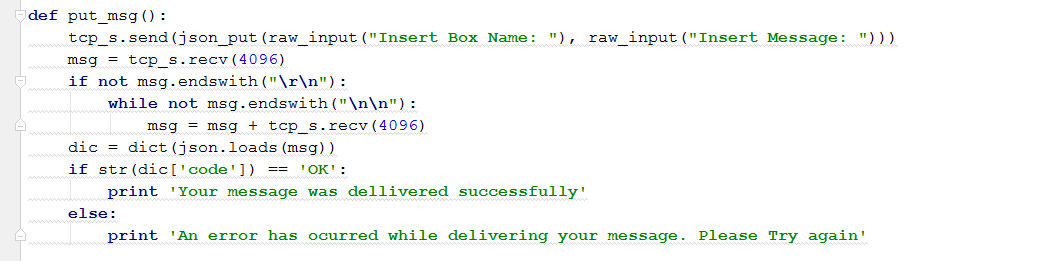
\includegraphics[width=400pt]{put_msg}
\caption{Função \textit{put\_msg}}
\label{fig:put_msg}
\end{figure}

Este módulo pede o nome da caixa para onde o utlizador quer enviar a mensagem e passa isso como argumento à função \textit{json\_put}, a qual vai criar uma \textit{string} de \textit{JSON}, com campos relativos ao tipo de função a ser executada (\textit{type}), ao nome da caixa para onde vai ser enviada a mensagem \textit{(name)} e a mensagem em si \textit{(content)}. 

\begin{figure}[h]
\center
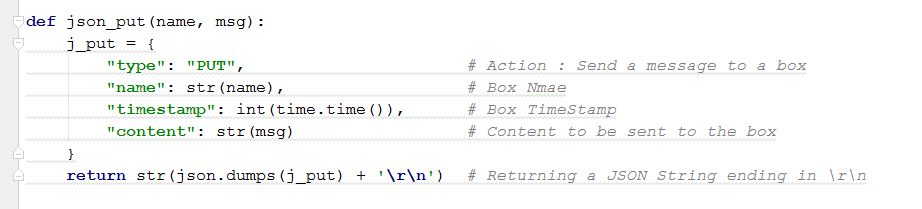
\includegraphics[width=400pt]{json_put}
\caption{Função \textit{json\_put}}
\label{fig:json_put}
\end{figure}

Após isto, a socket vai enviar a \textit{string} de \textit{JSON} acabada em \textbackslash r \textbackslashn e vai aguardar por uma resposta do \textit{server} também acabada em \textbackslash r \textbackslash n, e, após receber a resposta, apresenta ao utilizador uma mensagem de sucesso caso a mensagem tenha sido enviada. Caso contrário, mostra uma mensagem de erro com detalhes sobre o porquê de não ter sido possivel enviar a caixa.

\newpage
\FloatBarrier
\subsection{GET}
Na função \textit{GET} vai ser pedido ao \textit{server} o conteúdo de uma caixa. Para que tal seja possivel, criou-se o módulo \textit{get\_box} que pede ao utilizador o nome da caixa a que pretende aceder e usa-a sua resposta como argumento para a função \textit{json\_get}.

\begin{figure}[h]
\center
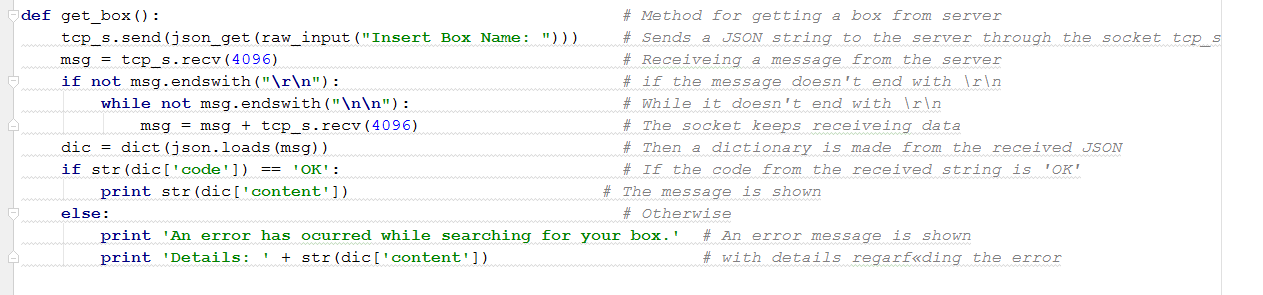
\includegraphics[width=400pt]{get_box}
\caption{Função \textit{get\_box}}
\label{fig:get_box}
\end{figure}

A partir deste ponto, gera uma string de \textit{JSON} com campos relativos ao tipo de função a ser executada (\textit{type}), nome da caixa (\textit{name}), tempo em segundos (\textit{timestamp}) e a assinatura do utilizador, que é feita com base na concatenação da chave pública, com o \textit{timestamp} e o nome da caixa, sendo depois assinada pelo método \textit{PKCS1\_PSS} com recurso à chave privada do utilizador

\begin{figure}[h]
\center
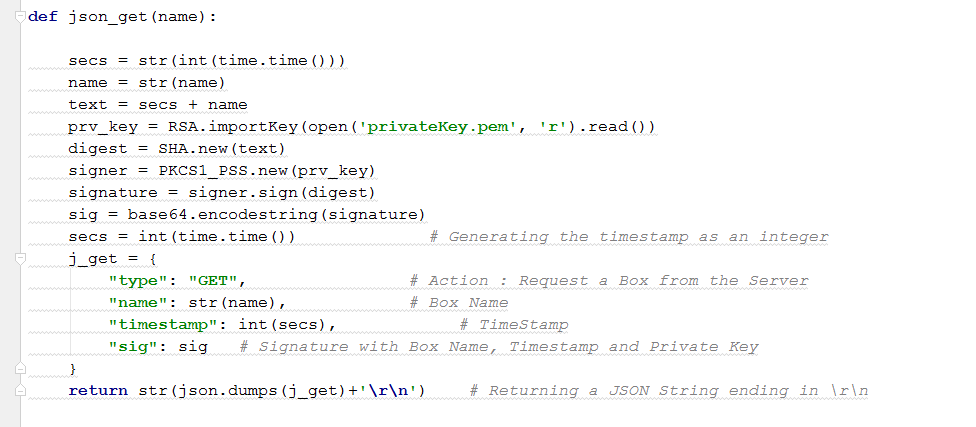
\includegraphics[width=400pt]{json_get}
\caption{Função \textit{json\_get}}
\label{fig:json_get}
\end{figure}

Depois disto, o \textit{socket} manda uma mensagem acabada em \textbackslash r \textbackslash n, à qual o servidor vai responder enviando também uma mensagem acabada em \textbackslash r \textbackslash n. Após isto, se a caixa existir, o programa mostra o conteúdo da mesma. Caso a caixa não exista ou esteja vazia, o programa vai mostrar uma mensagem de erro com detalhes sobre esse mesmo erro.

\newpage
\FloatBarrier
\chapter{Conclusões}
\label{chap.conclusao}
Nos dias de hoje, para que haja segurança e fiabilidade num programa que faça comunicações pela internet, é preciso que haja muito trabalho por trás. Este trabalho demonstrou as dificuldades que os programadores passam na criação de tais programas. Desde manter o \textit{server} e o cliente a trabalhar segundo os mesmo moldes, a evitar que a privacidade dos clientes seja posta em risco, tendo também especial consideração para que o programa não se comporte de maneira estranha (não prevista) face à passagem de argumentos estranhos (inválidos). Todos estes elementos são essenciais para que o utlizador do programa consiga ter uma boa experiencia aquando da sua utilização, mantendo sempre a sua privacidade.

Concluimos que, para garantir a fiabilidade de um programa é necessário olhar para o mesmo de diversas perspetivas (mesmo as que, provavelmente, seriam consideradas irracionais) para que seja possível tentar prever todos os casos que o programa em causa enfrentará. Cada situação imprevisivel levanta problemas e os testes exaustivos tentam ao máximo garantir que essas situação, simplesmente, não existem.
 

\chapter*{Contribuições dos autores}
\label{chap.contribuicao}
RS escreveu a maior parte do código, testes e do relatório

PV focou-se no relatório em \LaTeX e revisão textual.


No geral, distribui-se a percentagem de trabalho 70\% para RS e 30\% para PV.

\end{document}
